\documentclass[a4paper]{article}
\usepackage[utf8x]{inputenc}
\usepackage[slovene]{babel}
\usepackage{subfigure}
\usepackage{graphicx}
\usepackage{float}
\usepackage{hyperref}

\hyphenpenalty=5000
\tolerance=1000

\title{Analiza algoritma uniclass}
\author{Jure Ham - 63080514}
\maketitle

\begin{document}

\pagebreak

\section{Opis programa}
	Program uniclass je celovit paket namenjen testiranju in nadgradji algoritma uniclass. Grafi"cni vmesnik omogo"ca nalaganje testnih primerov, spreminjanje osnovnih nastavitev algoritma ter sproten prikaz delovanja. Ker je algoritem ra"cunsko zahteven, je program implementiran v javi, ki omogo"ca dober kompromis med hitrostjo izvajanja in hitrostjo razvoja.

	\subsection{Branje podatkov}
		Program podpira nalaganje testnih primerov v formatu tab, ki je osnoven format programskega paketa orange. Implementacija je omejena na zvezne in neurejene diskretne vrednosti ter na eno samo meta vrednost, ki postane ime entitete. \\
		Manjkajo"ci podatki so obravnavani kot posebne vrednosti, kar pomeni, da je razdalja med entiteto z vsemi podatki in entiteto brez podatkov najve"cja, razdalja med dvema entitetama brez podatkov pa je najmanj"sa. Razlog za to odlo"citev je zelo enostavna implementacija.
	
	\subsection{Ra"cunanje matrike razdalj}
		Razdaljo med dvema primeroma izra"cunamo kot vsoto vseh razdalj med atributi. V primeru, da je aribut diskreten in neurejen, je razdalja diskretna in sicer 0, "ce sta vrednosti enaki in 1, "ce sta vrenosti razli"cni. V primeru, da je atribut zvezen, pa se razdalja inra"cuna kot $$ dist = \left|\frac{value_1 - value_{min}}{value_{max} - value_1} - \frac{value_2 - value_{min}}{value_{max} - value_2}\right| $$
		Kjer je $value_1$ vrednost atributa pri prvem primeru, $value_2$ vrednost atributa pri drugem primeru, $value_{max}$ najve"cja vrednost atributa in $value_{min}$ najmanj"sa vrednost atributa.\\
		Vse razdalje se pomno"zijo "se s pomembnostjo atributa, ki je izra"cunana z algoritmom information gain in se lahko spreminja v grafi"cnem vmesniku, ter s pomembnostjo vrednosti, ki je definirana kot unikatnost vrednosti. Unikatnost izra"cunamo na diskretiziranih vrednostih in sicer tako, da izra"cunamo povre"cno "stevilo primerov z enako vrednostjo, nato pa to "stevilo delimo s "stevilom primerov, ki imajo enako vrednost kot primer, ki nas zanima. 
		$$ uni = \frac{\frac{\parallel E \parallel}{\parallel V_u \parallel}}{\parallel E_i=v \parallel} $$
		Kjer je $E$ mno"zica vseh entitet, $V_u$ mno"zica vseh unikatnih vrednosti za atribut in $v$ vrednost za katero ra"cunamo unikatnost.\\
		Ko primerjamo dva primera, je unikatnost dolo"cena kot produkt unikatnosti prve in druge vrednosti.
		
	\subsection{Simuliranje sil}
		Algoritem uniclass deluje tako, da primere predstavi kot delce v dvodimenzionalnem prostoru. Vsem delcem dodeli enako maso, nato pa med njimi ra"cuna sile, ki delce premikajo.
		\subsubsection{Vztrajnost}
			Za razliko od algoritma MDS, uniclass upo"steva tudi vztrajnost delcev. Vztrajnost ra"cunamo tako, da ima vsak delec poleg atributa pozicija tudi atribut hitrost, ki se spreminja glede na sile, ki nanj delujejo. S spreminjanjem mase delcev lahko uravnavamo kaoti"cnost sistema, saj je vpliv sil na hitrost delca obratno sorazmeren z njegovo maso. Za"cetna masa delcev je sorazmerna z vsoto vseh sil med delci, tako da kaoti"cnost sistema ni odvisna od testnih podatkov.
		\subsubsection{Izra"cun sile med delcema}
			Algoritem deli delce na podobne in na ne podobne. Podobni delci so tisti, med katerimi je mo"c povezave manj"sa od dolo"cene meje, ki je na za"cetku definirana kot povpre"cna mo"c povezave med vsemi delci, kasneje pa jo lahko preko uporabni"skega vmesnika tudi spreminjamo. Mo"c povezave je definirana kot $ 1 - razdalja $.\\
			Podobni delci se privla"cijo s silo, ki je definirana kot $ \frac{(f - k) * d^2}{C} $, kjer je $f$ mo"c povezave, $k$ je prej omenjena meja, $d$ je razdalja med delcema v prostoru, $C$ pa konstanta. \\
			Delci, ki si niso podobni, se odbijajo po formuli $ \frac{(f - k) * C}{d} $.\\
			Tako izra"cunana sila se nato "se deli z maso delca. Ker so razdalje lahko zelo majhne, je dolo"cena tudi najve"cja mo"zna sila, kar prepre"ci kaoti"cnost sistema.
		\subsubsection{Zaletavanje delcev}
			Ker algoritem predstavi primere kot delce z maso in radijem, ki je ve"cji od 0, se delci med seboj tudi zaletavajo. S tem prepr"cimo to, da bi se ve"c delcev zbralo na isti oziroma zelo podobni poziciji v prostoru, hkrati pa omogo"cimo zdru"zevanje podobnih delcev, kar bi bilo v nasprotnem primeru zaradi vztrajnosti skoraj nemogo"ce.\\
			Da se delci, ki si niso podobni, nebi zdru"zevali, definiramo togost delcev pri odboju kot obratno verdnost njune podobnosti. Tako dva zelo podobna delca po trku potujeta v skoraj enako smer, dva zelo razli"cna pa vsak v svojo.
		\subsubsection{Meje polja}
			Delci, ki z ostalimi primeri nimajo mo"cnih povezav, nam bodo hitro pobegnili izven vidnega polja, saj jih bo ve"cina delcev odbijala. Ta problem vsaj delno re"simo s tem, da okoli polja postavimo mejo, od katere se vsi delci odbijajo. Tako take delce ujamemo na robu polja, kjer se bodo posku"sali "cim bolj pribli"zati delcem, ki so jim podobni in "cim bolj oddaljiti od delcev, ki jih odbijajo. Da delci nebi ostali popolnoma prilepljeni na mejo, v algoritem uvedemo kr"cenje prostora, ki v vsakem ciklu ra"cunanja delce malo pomakne proti sredini. Razdalja za katero se delci premaknejo, je odvisna od oddaljenosti od sredi"s"ca.
	
	\subsection{Barvanje delcev}
		Za bolj"so preglednost delovanja delce pobarvamo glede na razred kateremu pripadajo. Razrede pobarvamo tako, da jih "cim bolj enakomirno razporedimo po robu barvnega kroga. \\
		Poleg barvanja razredov delcem dodelimo "se dve vizualni lastnosti. Prva lastnost je temnost, ki je odvisna od velikosti sile, ki deluje nanj, druga lastnost pa je rde"ca obroba, ki se poka"ze, kadar algoritem kNN iz pozicije delca v prostoru ni pravilno dolo"cil njegovega razreda.

\section{Vizualizacija podatkov}
	Ker algoritem uniclass obdeluje podatke v dvodimenzionalnem prostoru, je zelo primeren za vizualizacijo podatkov. S spreminjanjem nastavitev algoritma lahko v "zivo spremljamo kaj se s delci dogaja in pri tem izvemo zanimive lastnosti podatkov. Zaradi te lastnosti algoritma slika ne odseva vseh vizualnih lastnosti podatkov, je pa kljub temu informativna. \\
	Pri sliki \ref{f-derm-uni} lahko vidimo, da sta zelen in rumen razred dominantna, saj imata veliko mo"cno povezanih primerov, moder razred ima ravno tako veliko primerov, vendar le ti niso zelo enotni. To lastnost izvemo iz oblike lika, ki ga delci oblikujejo. Vijoli"cen razred je majhen, vendar relativno dobro povezan. Iz pozicije lahko sklepamo, da je nekoliko podoben rumenemu razredu, hkrati pa ima skupne lastnosti z nekaterimi "clani rde"cega razreda. Moder in rde"c razdred sta o"citno precej druga"cna od ostalih, vendar sta znotraj razreda tako slabo povezana, da se pozamezni primeri me morejo zdru"ziti v skupine. "Ce bi opazovali animacijo in ne le slike, bi lahko opazili "se, da se delci v zelenem razredu najhitreje giblejo, kar pomeni, da so sile med njimi najve"cje.\\
	Dejstvo, da se moder in rde"c razred ne zdru"zita v skupino je hkrat problem in prednost algoritma uniclass. Ker se nista zdru"zila lahko sklepamo, da so si primeri znotraj razreda precej razli"cni, hkrati pa ne moremo jasno videti v kateri razred spada kateri primer zaradi "cesar bi bila klasifikacija nerazporejenih primerov izredno zahtevna.\\
	Objektivno bi morda lahko ocenjevali kvaliteto vizualizacije s pono"cjo clusteringa, ki bi ga izvedli s pono"cjo pozicije delcev v prostoru. Ta metoda nam bi verjetno pokazala kako dobro dolo"cen algoritem razdeli podatke po dvodimenzionalnem prostoru, nebi nam pa povedala, kaj vse lahko o podatkih izvemo s pomo"cjo algoritma, kar je glavni cilj vizualizacije.\\
	Ker ima vsaka metoda svoje prednosti in slabosti, ne bomo ugotavljali kater algoritem je najbol"si, temve"c bomo priporo"cili uniclass kot dodatno orodje za iskanje zakonitosti v podatkih.
	
	\begin{figure}[H]
	\begin{center}
	\subfigure[FreeViz]{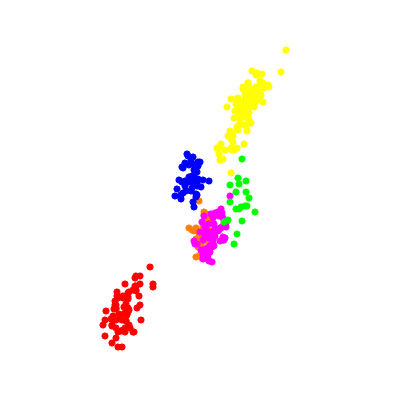
\includegraphics[width=0.5\textwidth]{img/der_freeviz.png}}
	\subfigure[MDS]{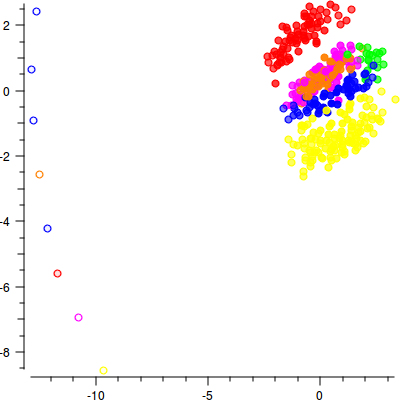
\includegraphics[width=0.5\textwidth]{img/der_mds.png}}
	\subfigure[uniclass]{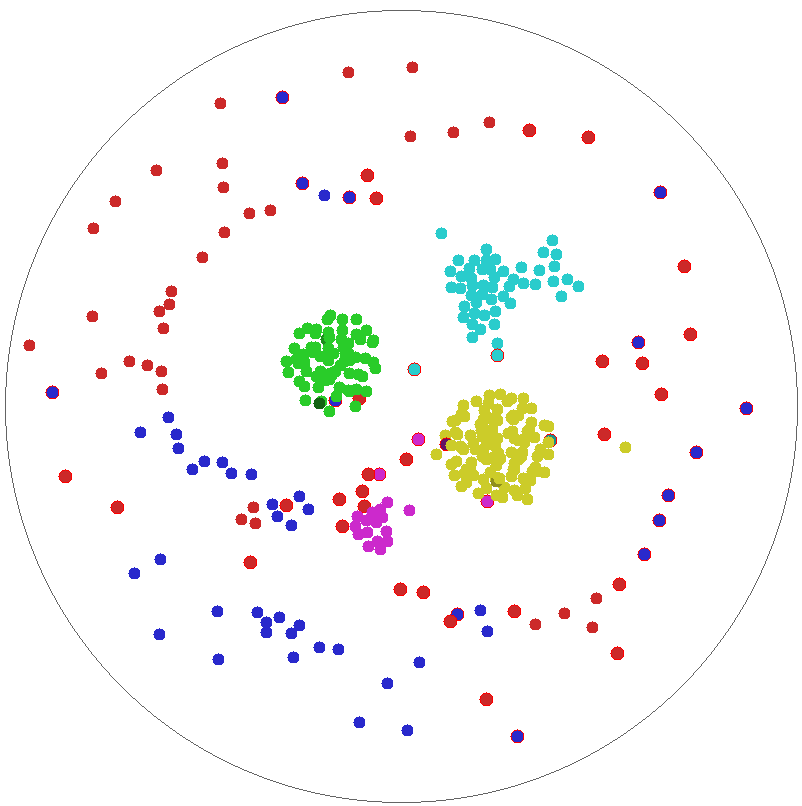
\includegraphics[width=0.6\textwidth]{img/der_uniclass.png}\label{f-derm-uni}}
	\end{center}
	\caption{Primerjava algoritmov za vizualizacijo na podatkih dermatology.tab. (Barve pri razli"cnih primerih ne predstavljajo nujno istega razreda.)}
	\label{f-derm}
	\end{figure}
	
\section{Klasifikacija}
	Poleg vizualizacije trenutna implementacija algoritma podpira tudi testiranje klasifikacijske to"cnosti algoritma. Razred primera se dolo"ci tako, da s pomo"cjo malo spremenjenega algoritma kNN iz najbli"zjih sosedov izberemo najbolj primernega kandidata. Za namene testiranja uporabimo princip izpusti enega(leave-one-out), kar pomeni, da poznamo razred vseh sosedov. Program pri tem nekoliko goljufa, saj ra"cuna pomembnost atributov tudi na tistem primeru, za katerega kasneje ugotavlja razred. \\
	Glavna mo"c algoritma uniclass pri klasifikaciji je vizualna komponenta, saj lahko sami vidimo v kak"sni okolici se nahaja dolo"cen primer. "Ce bi se na sliki \ref{f-zoo} naznan primer nahajal v sredini rde"ce skupine bi lahko z zagotovostjo trdili, da tja tudi spada. "Ce bi se nahajal nekje ob robu, pa bi lahko napovedali ve"c razli"cnih potencialnih razredov.\\
	Razdalja med primeri je dolo"cena kot kvadrat razdlaje med primeroma v prostoru. Poleg razdalje agoritem upo"steva tudi razpr"senost primerov, tako da se iskanje sosedov ustavi takoj, ko je razdalja do naslednjega primera ob"cutno ve"cja od trenutne povpre"cne razdalje. S tem prepre"cimo napa"cno klasifikacijo primerov, ki se nahajajo v zelo majhni skupi v bli"zini velike skupine. \\
	Na sliki \ref{f-zoo} lahko vidimo katere primere je algoritem pravilno klasificiral in katere napa"cno(rde"ca obroba). Klasifikacijska to"cnost za ta primer je 94\%.

	\begin{figure}[H]
	\begin{center}
	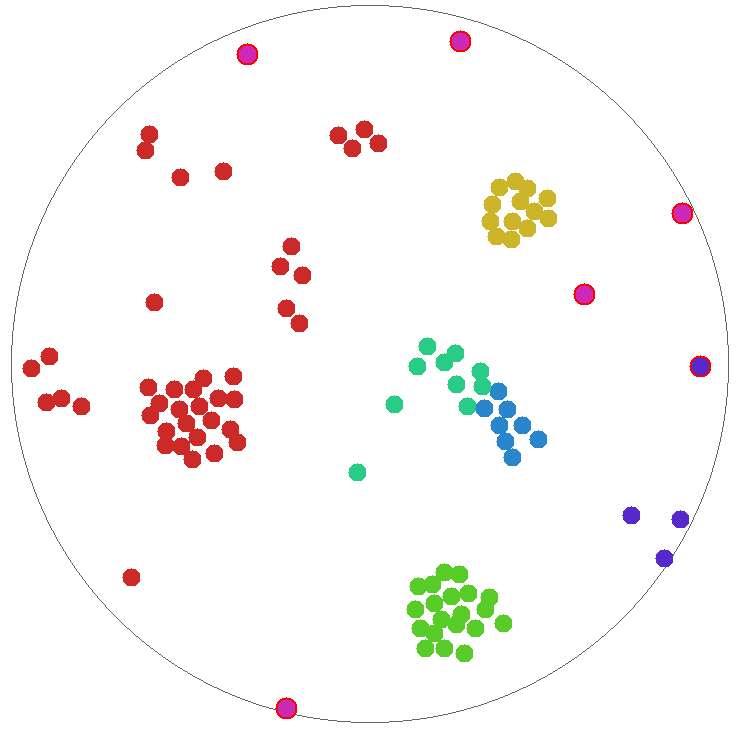
\includegraphics[width=0.8\textwidth]{img/zoo_uniclass.png}
	\end{center}
	\caption{Predstavitev podatkov zoo.tab z algoritmom uniclass.}
	\label{f-zoo}
	\end{figure}
	
	\subsection{Primerjava klasifikacijske to"cnosti}
		Za primerjavo klasifikatorjev sem si izbral "stiri popularne klasifikatorje. Pri interpretiranju rezultatov je potrebno upo"stevati tudi dejstvo, da je uniclass dela"c najpo"casnej"sa in najmanj avtomatska metoda, saj je za zglede klasifikacjske rezultate potrebno ro"cno nastaviti mejo tako, da so skupine primerov "cim bolj lo"cene. To se zdi kot goljufanje vendar ni, saj lahko vizualno lo"cimo skupine tudi, "ce poznamo razrede le majhnega "stevila primerov.\\

		\begin{tabular}{ | l | l | l | l | }
		\hline
		 & dermatology.tab & zoo.tab & heart.tab \\ \hline
		uniclass & 0.91 slika \ref{f-clas-der} & 0.94 slika \ref{f-zoo} & 0.82 slika \ref{f-clas-heart} \\ \hline
		Ve"cinski & 0.31 & 0.41 & 0.54 \\ \hline
		SVM & 0.97 & 0.95 & 0.83 \\ \hline
		Naivni Bayesov & 0.97 & 0.92 & 0.83 \\ \hline
		kNN & 0.96 & 0.97 & 0.77 \\ \hline
		\end{tabular}
		\\\\
		Iz zbranih podatkov lahko ugotovimo, da algoritem uniclass ni najmo"cnej"sa metoda, "ce "zelimo golo klasifikacijo. Poleg po"casnosti ima algoritem problem tudi s klasifikacijsko to"cnostjo. Zaradi teh ugotovitev priporo"camo funkcijo klasificiranja podatkov le kot pomo"c pri vizualizaciji podakov, kjer nam pri dolo"cenih primerih manjkajo podatki o razredu. 
		
	\begin{figure}[H]
	\begin{center}
	\subfigure[dermatology.tab]{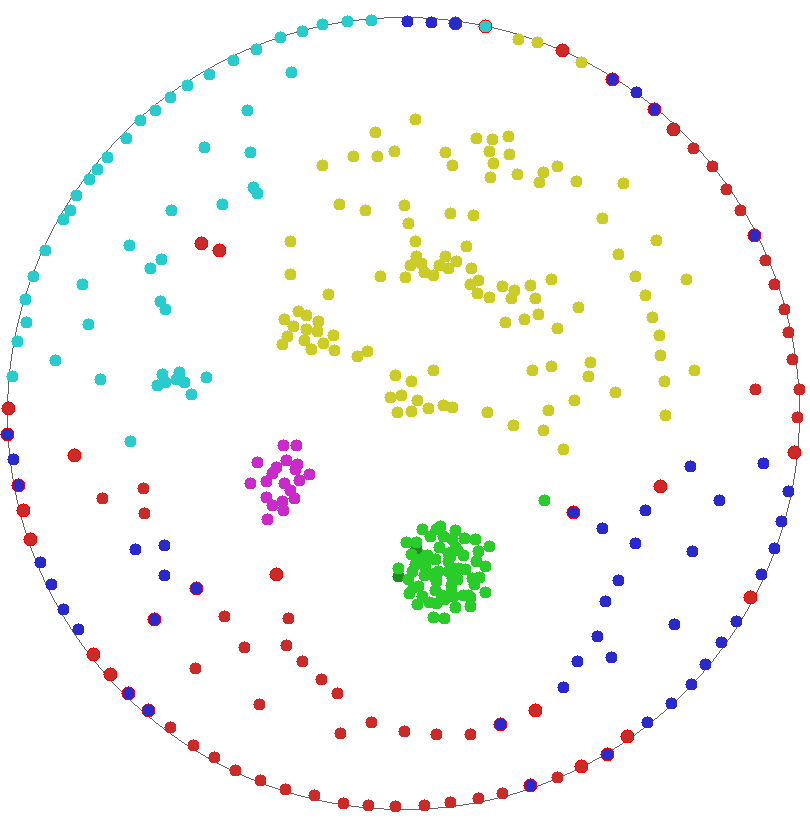
\includegraphics[width=0.5\textwidth]{img/der_uniclass_1.png}\label{f-clas-der}}
	\subfigure[heart.tab]{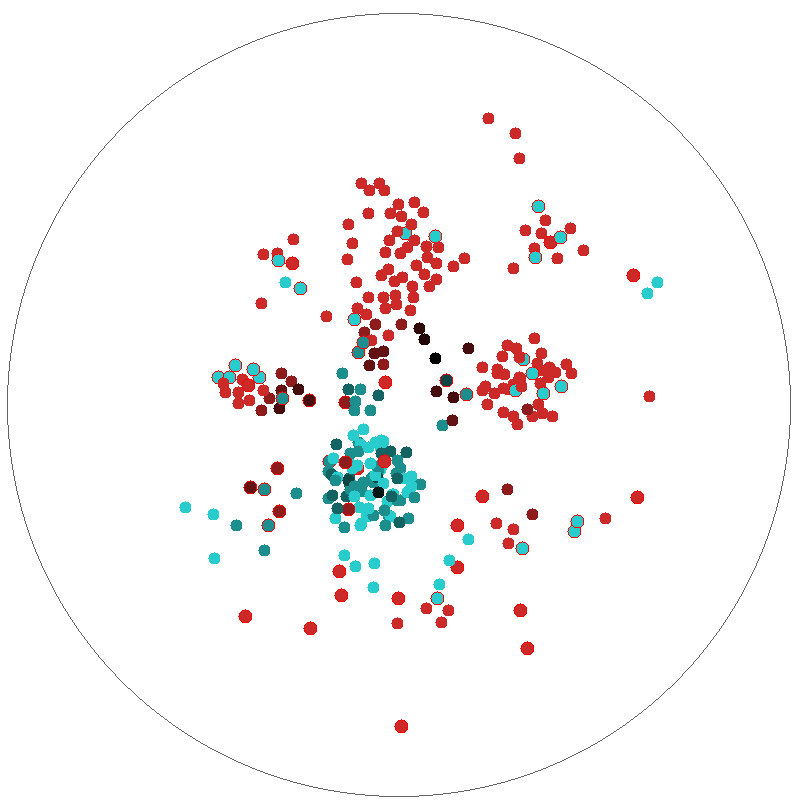
\includegraphics[width=0.5\textwidth]{img/heart_uniclass.png}\label{f-clas-heart}}
	\end{center}
	\caption{Klasifikacija podatkov z algoritmom uniclass.}
	\label{f-der-1}
	\end{figure}

\section{Clustering}
	Ker algoritem posamezne primere zdru"zuje v skupine najbolj podobnih, se mo"znost clusteringa zdi o"citna. Trenutna implementacija algoritma za izra"cun sil upo"steva tudi pomembnost atributov, za kar potrebujemo razrede, vendar grafi"cni umesnik podpira ponastavitev vseh atributov in s tem prepre"citev goljufanja. Ko atribute ponastavimo, ugotovimo da se kljub temu primeri skoraj enako dobro razporedijo po skupinah(slika \ref{f-der-2}). Ker program nima implementirane funkcije clusteringa, si bomo pomagali s paktom orange in sicer z vti"cnikoma k-Means Clustering ter Hierarchical clustering. 
	
	\begin{figure}[H]
	\begin{center}
	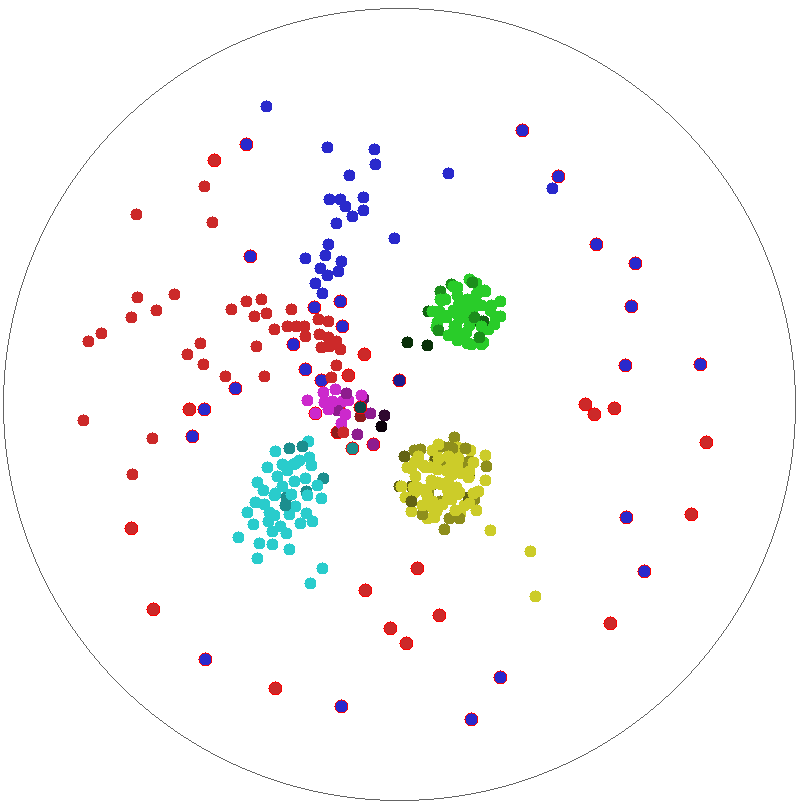
\includegraphics[width=0.6\textwidth]{img/der_uniclass_2.png}
	\end{center}
	\caption{Predstavitev podatkov dermatology.tab brez upo"stevanja pomembnost atributov.}
	\label{f-der-2}
	\end{figure}

	\subsection{Primerjava algoritmov}
		Za primerjavo algoritmov smo si izbrali podatke zoo.tab. V programi uniclass smo ponastavili pomomebnost atributov ter dobili sliko \ref{clus-uni-img}. Podatke smo izvozili tako, da smo imeli poleg podatka o razredu le podatek o poziciji, ter jih uvozili v paket orange. Nato smo uvozili "se originalne podatke, ter jih za prvo primerjavo poslali v widget k-Means Clustering, ki smo ga nastavili tako, da si je sam izbral optimalno "stevilo clusterjev. Na sliki \ref{clus-uni-kmeans} si lahko ogledate rezultate clusteringa z uporabo algoritma uniclass, na sliki \ref{clus-kmeans-solo} pa rezultate pridobljene le z uporabo algoritma k-Means. Opazimo lahko, da je algoritem uniclass bolje razporedil sesalce, ostali razredi pa so razporejeni podobno dobro.\\
		Za drugo primerjavo smo podatke obdelali z algoritmom hierarchical clustering, pri ra"cunanju povezav pa smo uporabili wardovo povezavo. Ker algoritem od nas zahteva, da sami nastavimo mejo za lo"citev razredov, rezultati niso odvisni le od algoritmov, vendar tudi od raziskovalca. Na sliki \ref{clus-uni-hier} si lahko ogledate rezultate pridobljene s pomo"cjo algoritma uniclass, na sliki \ref{clus-hier-solo} pa rezultate brez uniclassa. Rezultati so si zopet zelo podobni. Pri uporabi uniclass smo napa"cno zdru"zili insekte in nevreten"carje, brez uniclassa pa dvo"zivke in nevreten"carje. \\
		Ker so rezultati zelo podobni, smo primerjali "se clustering na podatkih dermatology.tab(Slika \ref{clus_der}), kjer se je algoritem uniclass dobro obnesel. \\
		Pri primerjavi rezultatov se je podtrebno zavedati, da algoritem uniclass za dobre rezultate zahteva od uporabnika ro"cno nastavitev parametrov, kar onemogo"ci popolnoma objektivno primerjavo. 

	\begin{figure}[H]
	\begin{center}
	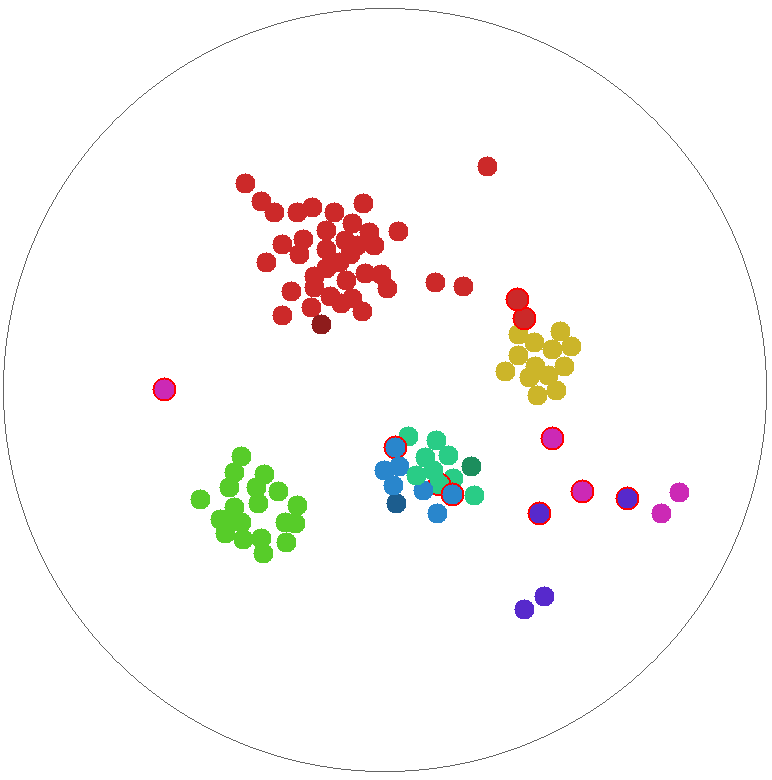
\includegraphics[width=1\textwidth]{img/clus_uni_pic.png}
	\end{center}
	\caption{Podatki zoo.tab v programu uniclass brez ocene atributov.}
	\label{clus-uni-img}
	\end{figure}

	\begin{figure}[H]
	\begin{center}
	\subfigure[Z uniclass]{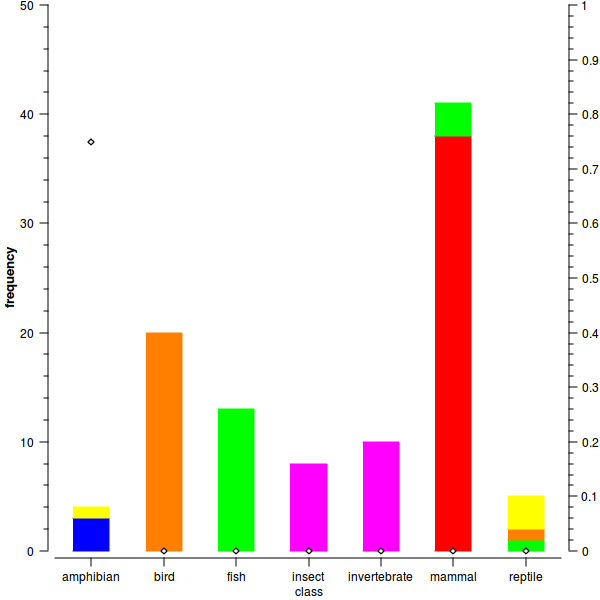
\includegraphics[width=0.75\textwidth]{img/clus_uni_kmeans.png}\label{clus-uni-kmeans}}
	\subfigure[Brez uniclass]{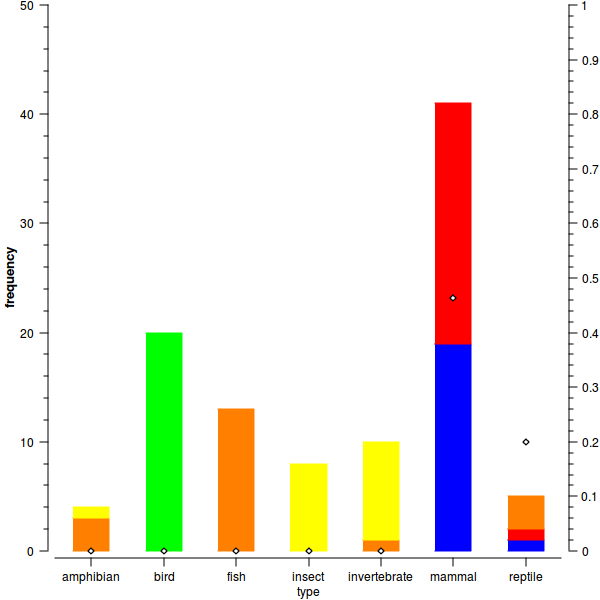
\includegraphics[width=0.75\textwidth]{img/clus_kmeans.png}\label{clus-kmeans-solo}}
	\end{center}
	\caption{Primerjava clusteringa podatkov z uporabo algoritma k-Means Clustering}
	\label{clus-kmeans}
	\end{figure}
	
	\begin{figure}[H]
	\begin{center}
	\subfigure[Z uniclass]{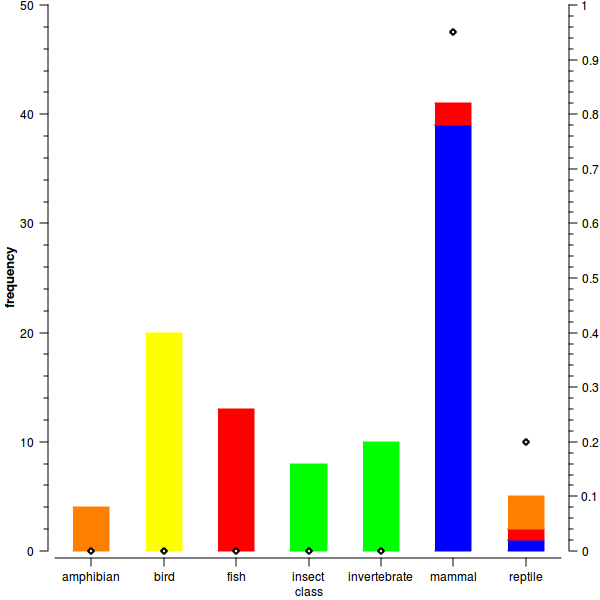
\includegraphics[width=0.75\textwidth]{img/clus_uni_hier.png}\label{clus-uni-hier}}
	\subfigure[Brez uniclass]{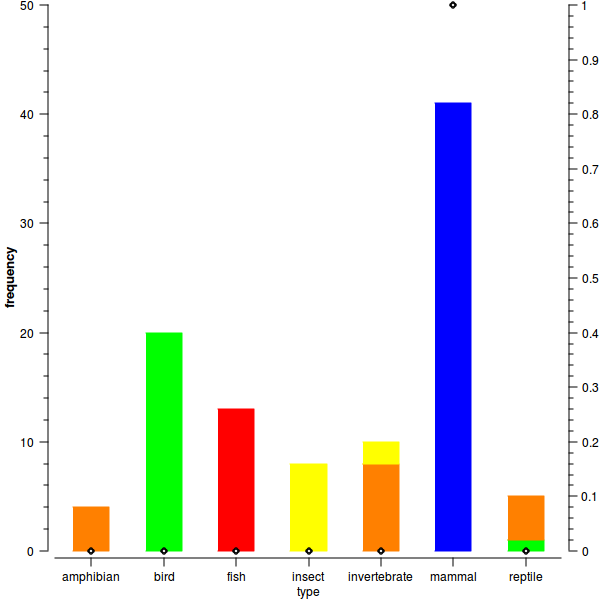
\includegraphics[width=0.75\textwidth]{img/clus_hier.png}\label{clus-hier-solo}}
	\end{center}
	\caption{Primerjava clusteringa podatkov z in brez uporabe algoritma Hierarchical clustering.}
	\label{clus-hier}
	\end{figure}
	
	\begin{figure}[H]
	\begin{center}
	\subfigure[Z uniclass]{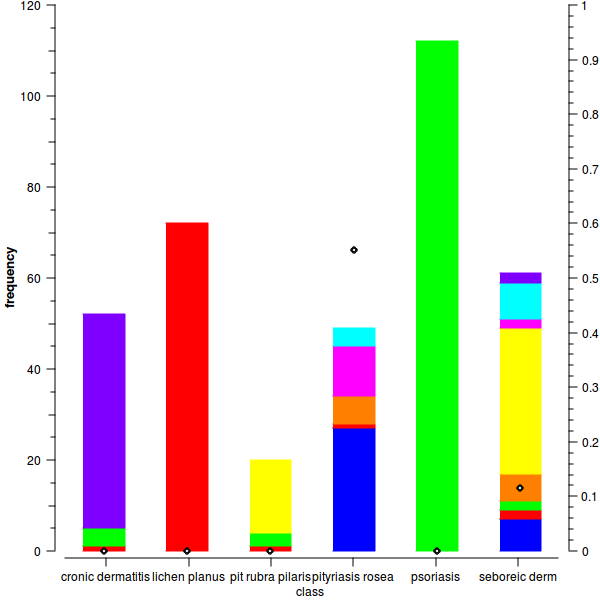
\includegraphics[width=0.75\textwidth]{img/clus_uni_kmeans_der.png}\label{clus-uni-der}}
	\subfigure[Brez uniclass]{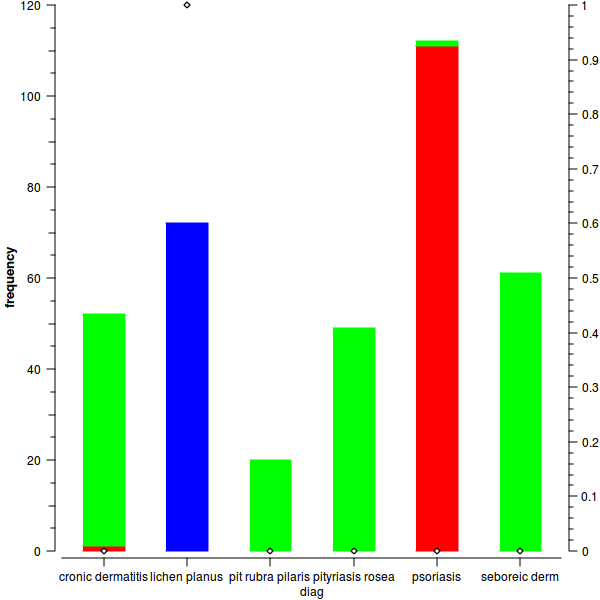
\includegraphics[width=0.75\textwidth]{img/clus_kmeans_der.png}\label{clus-der}}
	\end{center}
	\caption{Primerjava clusteringa podatkov dermatology.tab z in brez uporabe algoritma Hierarchical clustering.}
	\label{clus_der}
	\end{figure}

\section{Zaklju"cek}
	Skozi seminarsko nalogo smo se dotaknili treh potencialnih aplikacij algoritma uniclass. Ugotovili smo, da je najve"cja mo"c algoritma v vizualizaciji podatkov, saj omogo"ca dodatno perspiktivo pri opazovanju podatkov. Poleg opazovanja razpr"senosti podatkov lahko s pomo"cjo opazovanja premikanja lo"cimo mo"cno in "sibko povezane primere. S spreminjanjem nastavitev v grafi"cnem umesniku pa lahko v "zivo opazujemo spremembe, kar nam omogo"ca odkrivanje bolj skritih zakonitosti in vzorcev(slika \ref{f-votes}). \\
	Tudi pri clusteringu podatkov se algoritem dobro obnese, saj zelo u"cinkovito zmanj"sa "stevilo atributov protrebnih za podobno kvalitetne rezultate. 

	\begin{figure}[H]
	\begin{center}
	\subfigure[Meja postavljena nizko]{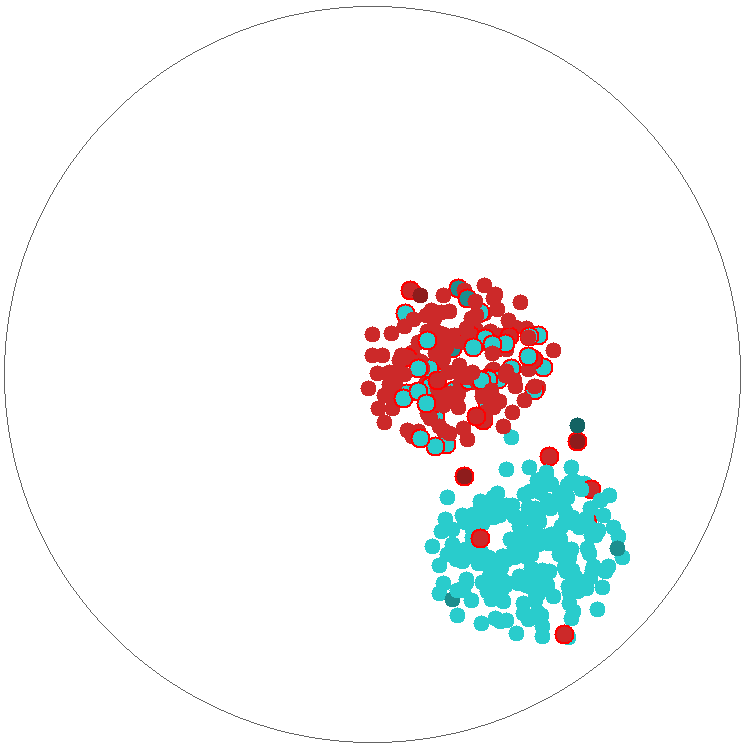
\includegraphics[width=0.6\textwidth]{img/vote_1.png}}
	\subfigure[Meja postavljena visoko]{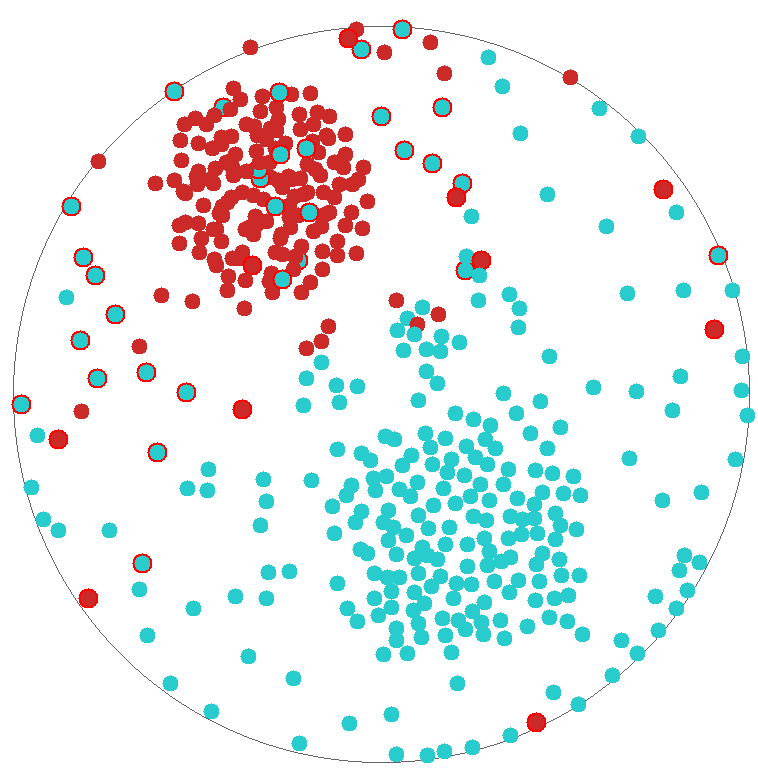
\includegraphics[width=0.5\textwidth]{img/vote_2.png}}
	\end{center}
	\caption{Opazovanje podatkov votes.tab, kjer lahko pri nizko postavljeni meji vidimo, da je med demokrati veliko takih, ki glasujejo podobno kot republikanci, pri visoko postavljeni meji, pa vidimo, da so si republikanci veliko bolj enotni kot demokrati.}
	\label{f-votes}
	\end{figure}

\section{Povezave}
	\href{https://github.com/hamaxx/Universe-Classification}{Izvorna koda projekta ter vsi testni primeri.}

\end{document}
